\chapter{Analýza}
\label{sec:an}

\section{Struktura systému}
\label{sec:an_struct}

Struktura celého systému je naznačena na obrázku \ref{fig:basic_struct}. Podřízené systémy komunikují s~nadřazeným na základě událostí. Nadřazený systém tyto události zpracovává a upravuje podle nich stav garáží v~evidenci. 

Zaznamenané události jsou také uchovávány v~historii událostí, spolu s~dalšími metadaty jako čas přijetí nebo původce.

Komunikace mezi podřízeným a nadřazeným systémem je postavena na modelu \textit{client/server}. Nadřazený systém provozuje server zvoleného protokolu (viz sekce \ref{sec:an_protocol}), ke kterému se podřízené systémy připojují. Komunikaci tedy vždy iniciuje podřízený systém. S~možností zasílání nevyžádaných zpráv podřízeným systémům v~této práci nepočítám, mohl by to však být námět pro další rozšíření.

Další, kdo přistupuje do systému, je uživatel. Přes webové rozhraní může sledovat stav garáží a historii událostí. Také zde může spravovat klíče, které slouží pro přístup ke komunikačnímu API systému. Přístup do webového rozhraní je zabezpečen heslem.

\begin{figure}[h!]
    \centering
    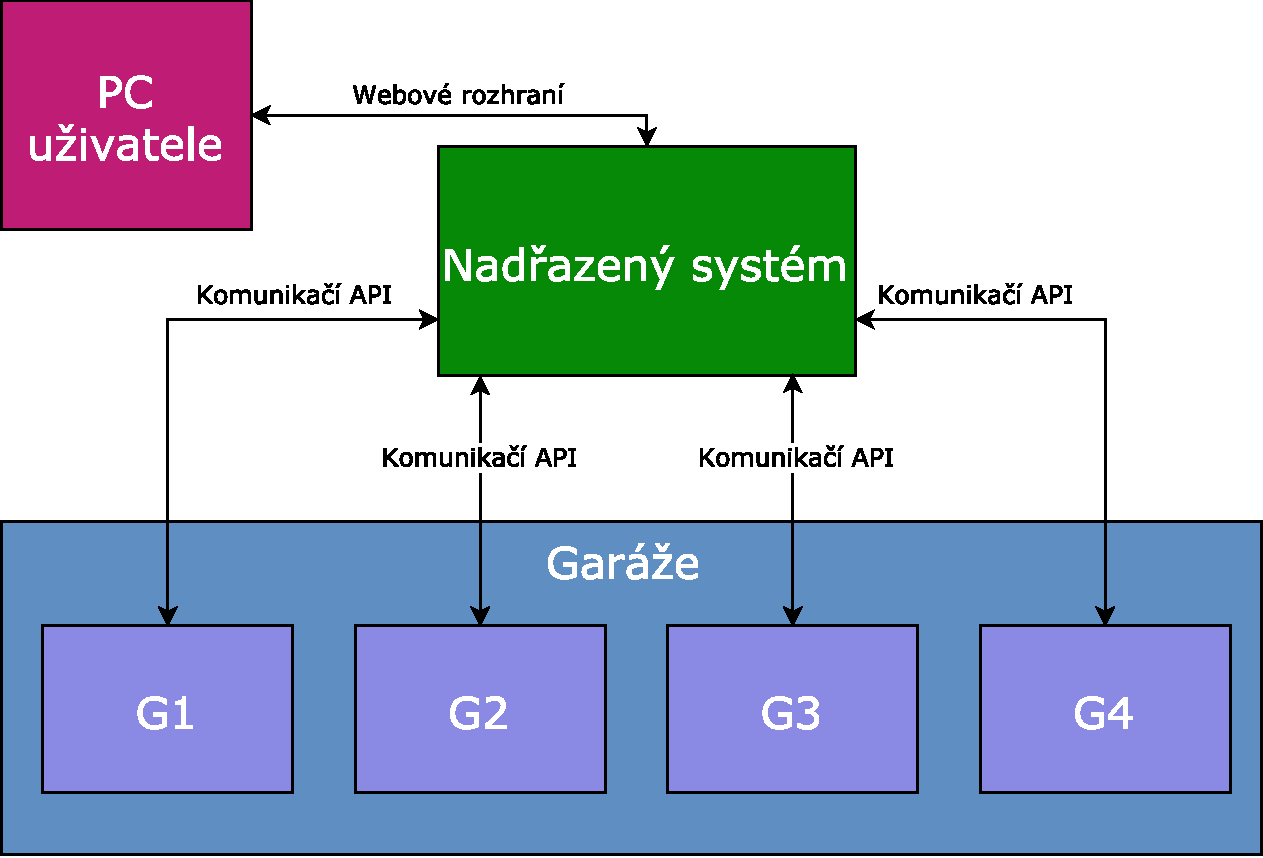
\includegraphics[width=0.7\textwidth]{images/basic_struct.pdf}
    \label{fig:basic_struct}
    \caption{Základní struktura systému}
\end{figure}

\subsection{Podřízený systém}

Podřízený systém je zařízení umístěné v~každé garáži, které sleduje stav okolí pomocí těchto senzorových vstupů:

\begin{itemize}
    \item teplota,
    \item světelá intenzita (fotobuňka),
    \item detekce kouře,
    \item detekce pohybu,
    \item stav dveří.
\end{itemize}

V~případě překročení mezních hodnot se zařízení okamžitě hlásí nadřazenému systému. Kromě toho také v~pravidelných intervalech odesílá kontrolní hlášení. 

Vyhodnocení události je provedeno nadřazeným systémem. Podřízený systém tedy hlásí každou událost (například otevření dveří), aniž by nějak zkoumal její závažnost.

Základní požadavek na podřízený systém je schopnost komunikace přes Ethernet či WiFi pomocí protokolu zvoleného v~sekci \ref{sec:an_protocol}. Kromě toho může být hardware prakticky libovolný.

\section{Výběr komunikačního protokolu}
\label{sec:an_protocol}

Nejdřív je nutné určit způsob komunikace, který bude systém používat. Díky tomu se budu při vybíraní platformy moci ujistit, že jsou dostupné vhodné knihovny a další software. 

Nadřazený systém bude se svými klienty (monitorovací zařízení v~jednotlivých garážích) komunikovat přes WiFi nebo Ethernet. Základem komunikace bude TCP/IP protokol, je však potřeba zvolit vhodný protokol z~aplikační vrstvy OSI modelu, který na něm bude stavět.

\subsection{Vlastní protokol}

Jedna z~možností je implementovat vlastní protokol pomocí TCP/IP socketů. Toto řešení se mi však nezdá příliš vhodné, neboť nepřináší žádné významné výhody, naopak se s~ním pojí řada komplikací.

Pro vlastní protokol by bylo nutné vytvořit robustní server, který zvládá obsluhu více klientů najednou. Dále by vzhledem k~citlivosti přenášených dat bylo nutné implementovat nějakou formu šifrování. Tyto velmi obsáhlé problémy přitom řeší většina dnešních protokolů.

Další nevýhodou je nutnost implementace klientské části protokolu při vytváření nových zařízení spravovaných nadřazeným systémem. To do jisté míry omezuje jeho rozšiřitelnost.

\subsection{HTTPS}
\label{sec:an_https}

Další možnost je využít ke komunikaci protokol HTTPS. V~tomto případě by klienti komunikovali se sytémem pomocí HTTP metod jako například \verb|get| nebo \verb|post|.

Jelikož součástí požadavků na systém je i webové uživatelské rozhraní, bude v~každém případě nutné použít webový server pro jeho provoz. Ten by pak bylo možné využít i k~poskytnutí API pro komunikaci systému s~garážovými čidly.

Vhodný webový server (jako například \textit{Nginx}) zajistí vícevláknovou obsluhu všech klientů. Protokol se také postará o~kryptografické zabezpeční přenášených dat, je však nutné získat certifikát k~ověření pravosti serveru (viz sekci \ref{sec:an_certs}).

Certifikát bude potřeba zajistit i v~případě, že komunikace s~klienty nebude postavena na tomto protokolu. Je totiž nutné také zabezpečit webové rozhraní, například kvůli ověření identity uživatele. Nutnost pořízení certifikátu tedy nepředstavuje nevýhodu oproti jiným protokolům. 

API realizované pomocí tohoto protokolu je poměrně snadno rozšiřitelné. Pro nově implementovanou operaci stačí definovat URL a případně formát přenášených dat.

Výhodou je také snadná implementace na straně klienta, tedy garážového čidla. Knihovny realizující klientskou část protokolu jsou dostupné na většině populárních platforem jako například \textit{Arduino} (s~Ethernet shieldem, oficiální knihovna \textit{EthernetClient} \cite{ard_web}) nebo \textit{ESP8266} (knihovna \textit{esp8266wifi} \cite{esp_web}).

\subsubsection{Certifikáty pro provoz HTTPS}
\label{sec:an_certs}

Pro provoz HTTPS serveru lze použít například certifikáty certifikační autority Let's Encrypt, které jsou poskytovány  zdarma. Kromě toho dodává Let's Encrypt také automatizačního klienta \textit{Certbot} \cite{certbot} pro snadné nasazení a aktualizaci jejich certifikátů. Bohužel certifikáty jsou vydávány pouze na doménu \cite{lets_encrypt_faq}, což komplikuje použití v~místní síti.

Jiná možnost je použití \textit{self-signed} certifikátu. Tento certifikát není podepsaný žádnou certifikační autoritou, ale pouze vlastníkem certifikátu. Může tedy sloužit k~šifrování komunikace (poskytuje veřejný klíč), ale je zranitelný vůči \textit{man-in-the-middle} útoku \cite{cert_wallen}.

\textit{Self-signed} certifiát však lze použít k~šifrování komunikace na uzavřené lokální síti, za předpokladu, že je server s~certifikátem (přesněji s~jeho soukromým klíčem) dostatečně zabezpečen \cite{cert_wallen}. 

Nevýhodou tohoto řešení je nedůvěra webových klientů (certifikát není podepsán certifikační autoritou), což by ovlivnilo přístup k~uživatelskému rozhraní a API systému. V~případě webového rozhraní by prohlížeč zobrazil varování o~neznámém certifikátu. To by však mohl uživatel ignorovat. 

Podřízené systémy by při zasílání požadavků museli přeskočit krok ověření totožnosti serveru. Jak toho dosáhnout v~knihovně \textit{Requests} pro Python (dostupné i pro \textit{Raspberry Pi}), je naznačeno v~ukázce \ref{lst:req_selfsigned}.

\begin{listing}[htbp]
\caption{\label{lst:req_selfsigned} Vytvoření HTTPS požadavku v~knihovně \textit{Requests}, bez verifikace serveru}
\begin{minted}[bgcolor=codebg]{python}
>>> import requests
>>> r = requests.get('https://testserver/test', verify=False)
>>> r.status_code
200
\end{minted}
\end{listing}

\subsubsection{Autentizace klientů na HTTPS}

Přístup k~API nadřazeného systému by měl být povolen pouze ověřeným klientům. Díky tomu bude možné zabránit například zasílání nepravdivých informací z~neznámých zdrojů.

Jednoduchou autentizaci přes HTTPS lze realizovat například pomocí generování API klíčů. Pro každý podřízený systém bude vygenerován klíč, kterým se při zasílání požadavku systém prokáže. Seznam platných klíčů by byl udržován v~databázi nadřazeného systému. Klíče by uživatel mohl přidávat nebo odebírat (například v~případě odcizení podřízeného systému) pomocí webového rozhraní.

Tyto klíče by také bylo nutné nahrát a uchovávat na podřízených systémech. Detaily tohoto procesu by záležely na platformě těchto systému. Například u~\textit{Arduina} by šlo klíč nahrát z~uživatelova počítače pomocí sériové linky (s~USB převodníkem) a udržovat ho v~EEPROM.

Také by bylo možné implementovat v~nadřazeném systému \uv{registrační mód}, který by bylo možné dočasně povolit ve webovém rozhraní. V~tomto módu by systém po přijetí speciálního API požadavku vygeneroval nový klíč. Ten by si uložil do své databáze platných klíčů, a také ho v~odpovědi zaslal žádajícímu zařízení. Pokud by mód povolen nebyl, odpovědel by systém chybovým kódem, například 403 -- \textit{Forbidden}. Zaslání požadavku z~podřízeného systému mohlo být provedeno stisknutím tlačítka.

Tento přístup by byl pravděpodobně uživatelsky příjemnější, přináší však potencionální bezpečnostní rizika. Například pokud by uživatel zapomněl mód vypnout, systém by byl otevřený k~registraci nežádoucích zařízení. Takový problém by se však dal řešit například automatickou deaktivací módu po uplynutí časového limitu.

Útočník snažící se získat klíč k~API by také mohl periodicky zkoušet registrační požadavek a čekat na aktivaci módu. Obrana proti tomuto útoku by byla složitější, šlo by například filtrovat IP adresy s~příliš častými požadavky.

Obecně vycházím z~toho, že i v~případě registrace nežádoucího zařízení nemůže toto zařízení krátkodobě způsobit výraznější škody -- do databáze nadřazeného systému může pouze zasílat nová data, která jsou navíc vázana k~jeho identitě (API klíči). Nemůže tedy získávat data od jiných podřízených systému či měnit jejich záznamy. Neautorizované zařízení se také objeví v~seznamu registrovaných API klíčů, kde může být snadno odhaleno. 

\subsection{MQTT}
\label{sec:an_mqtt}

MQTT je komunikační protokol založený na modelu \textit{publisher/subscriber}, vhod\-ný pro použití v~prostředí s~omezenými zdroji (malý výkon procesoru, omezená paměť atd.) \cite{mqtt_valerie}.

Komunikace mezi jednotlivými klienty v~systému je zprostředkována pomocí centrály, nazývané \textit{broker}. Ta spravuje adresy -- \textit{topics} -- na kterých mohou klienti publikovat či odebírat zprávy.

\begin{figure}[h!]
    \centering
    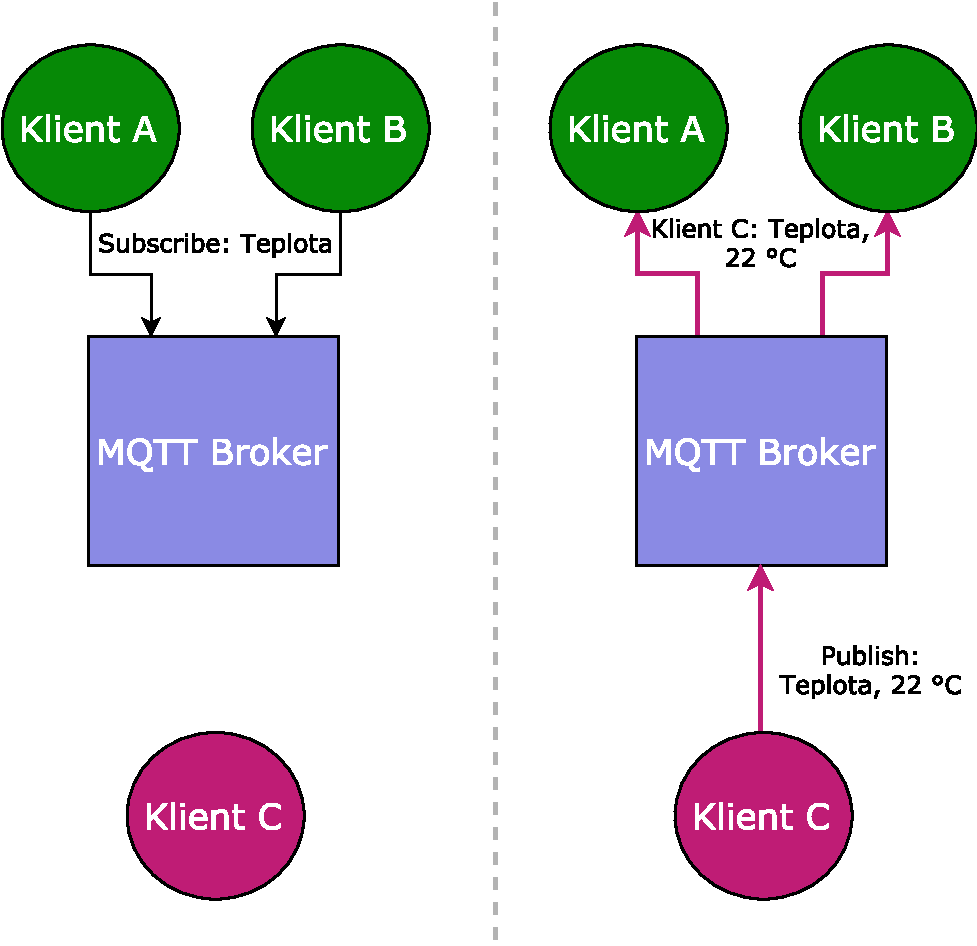
\includegraphics[width=0.7\textwidth]{images/basic_mqtt.pdf}
    \label{fig:basic_mqtt}
    \caption[Příklad struktury protokolu MQTT]{Příklad struktury protokolu MQTT \cite{mqtt_eclipse}}
\end{figure}

Na obrázku \ref{fig:basic_mqtt} tedy klienti \textcolor{green}{A} a \textcolor{green}{B} začnou odebírat (\textit{subscribe}) \textit{topic} \uv{Teplota}. Když pak klient \textcolor{magenta}{C} pak publikuje zprávu na tuto adresu, \textcolor{blue}{\textit{broker}} se postará o~doručení všem odebírajícím klientům.

Adresy je možné hierarchicky strukturovat. Lze tedy tvořit skupiny, například \verb|/senzory/obyvak/teplota| nebo \verb|/senzory/kuchyne/vlhkost|. Zprávy je nutné publikovat na jednoznačnou adresu, při odebírání je však možné použít modifikátory \verb|+| a \verb|#| pro specifikování skupiny adres. Modifikátor \verb|+| odpovídá libovolnému jednomu stupni hierarchie, \verb|#| pak libovolnému počtu libovolných stupňů. Pro odebírání všech senzorů vlhkosti lze tedy použít adresu \verb|/senzory/+/vlhkost|. Všechna data by pak bylo možné odebírat na adrese \verb|/senzory/#|. \cite{mqtt_eclipse}

V~případě této práce by tedy jak nadřazený systém, tak podřízené systémy byly klienty \textit{brokeru}. Podřízené systémy by publikovali naměřená data, která by nadřazený systém odebíral. Samotný \textit{broker} by pak mohl běžet souběžně s~nadřazeným systémem na zvolené platformě (například open-source \textit{broker Mosquitto} je dostupný na řadě platforem, včetně \textit{Raspberry Pi} \cite{mqtt_mosquitto_wiki}).

Protokol podporuje tři možnosti QoS (\textit{Quality of Service}) \cite{mqtt_valerie}:

\begin{itemize}
    \item Nejvýše jedno doručení -- tento mód pouze odešle zprávu, není zahrnut žádný opakovací mechanismus pro případ nedoručení.
    \item Alespoň jedno doručení -- v~tomto módu je zaručeno doručení zprávy, ta však může být doručena vícekrát.
    \item Přesně jedno doručení -- zde je ošetřeno i duplicitní doručování zpráv.
\end{itemize}

Použití sofistikovanějších metod doručení má vliv na výkon, a proto se v~některých případech vyplatí zvolit nižší úroveň QoS (například při posílání idempotentních zpráv). Pro tuto práci bych však pravděpodobně zvolil záruku přesně jednoho doručení.

\subsubsection{Šifrování a autentizace na MQTT}

V~této části se budu zabývat prostředky pro šifrování komunikace, které jsou dostupné v~\textit{brokeru} \textit{Mosquitto}.

První možnost je pro zabezpečení komunikace využít certifikáty, podobně jako u~HTTPS. Zde by se pravděpodobně také využil \textit{self-signed} certifikát (blíže popsaný v~sekci \ref{sec:an_certs}). \textit{Mosquitto} navíc také vyžaduje kořenový certifikát certifikační autority \cite{mqtt_mosquitto_tsl}. Při použití \textit{self-signed} ceritifikátů by bylo nutné tuto autoritu vytvořit a používané certifikáty u~ní podepsat (pro bližší informace viz \cite{ca_nguyen}). Kořenový certifikát by také bylo nutné distribuovat klientům.

Kromě certifikátů lze pro šifrování použít i PSK (\textit{pre-shared key}). V~tom případě \textit{broker} a jeho klienti používají pro zašifrování komunikace společný klíč (známý jak klientovi, tak \textit{brokeru}). Různí klienti přitom mohou mít různé klíče. \cite{mqtt_mosquitto_conf}

Bohužel podpora PSK v~MQTT klientech není příliš rozšířená. PSK je možné použít v~knihovně \textit{libmosquitto}, určené pro C/C++ (s~vazbami pro Python). U~této knihovny se mi však podařilo najít pouze manuálovou stránku (viz \cite{libmosquitto_man}), bez informací o~jejím dalším vývoji či udržování. Modul poskytující vazby do Pythonu byl nicméně předán projektu \textit{Paho} \cite{mosquitto_python}.

\textit{Paho} poskytuje implementace MQTT klientů pro mnoho platforem (včetně například \textit{Arduina} \cite{paho_embedded}). Dokumentace klientů pro C++ a Python však možnost šifrování pomocí PSK vůbec nezmiňuje \cite{paho_cpp_doc} \cite{paho_pyt_doc}.

Tyto možnosti lze použít i k~autentizaci klientů \textit{brokeru}. Při použití certifikátů lze v~konfiguračním souboru \textit{Mosquitta} zvolit \verb|require_certificate|. Poté bude od klienta vyžadován certifikát prokazující jeho totožnost. Při použití PSK lze k~autentizaci využít sdílený klíč (\textit{broker} odmítne klienty s~neplatnými klíči). Kromě toho je možno použít také autentizaci pomocí uživatelského jména a hesla, která je součástí MQTT protokolu, případně klienty neověřovat vůbec (a pouze šifrovat komunikaci). \cite{mqtt_mosquitto_conf}

\subsection{Závěr výběru protokolu}

V~sekcích \ref{sec:an_https} a \ref{sec:an_mqtt} jsem se blíže podíval na dva poměrně rozšířené protokoly aplikační vrstvy, které by bylo možné použít pro tvorbu nadřazeného systému.

Pokud by mezi požadavky na systém bylo zahrnuto zasílání nevyžádaných zpráv podřízeným systému (jak je zmíněno v~sekci \ref{sec:an_struct}), zvolil bych pravděpodobně protokol MQTT. V~tom je tato funkcionalita velmi snadno implementovatelná -- stačí aby podřízené systémy odebíraly \textit{topic}, na kterém by nadřazený systém publikoval zprávy.

Jelikož se však v~této práci zabývám systémem, který zprávy pouze přijímá a zaznamenává, rozhodl jsem se pro HTTPS. Nasazení tohoto protokolu je o~něco snazší (není potřeba na zařízení instalovat \textit{broker} a zařizovat certifikační autoritu -- stačí \textit{self-signed} certifikát) a s~jeho použitím mám více zkušeností. Také se částečně uvolní požadavky na volbu platformy (webový server bude potřeba v~každém případě, při volbě HTTPS jako komunikačního protokolu mezi systémy tedy nebude nutný žádný další software). 

Každopádně bude mým cílem navrhnout výslednou aplikaci tak, aby rozhraní pro podřízené systémy realizované pomocí HTTPS bylo možné snadno nahradit MQTT rozhraním.

K~zabezpečení komunikace (včetně webového rozhraní) použiju \textit{self-signed} certifikát. Hlavní důvod je požadavek na použití v~místní síti, bez zaručeného přístupu k~internetu. Toto rozhodnutí nemá vliv na návrh a implementaci systému, pouze na jeho nasazení. 

Pokud má provozovatel systému k~dispozici doménu a veřejnou IP, může k~zabezpečení použít certifikát podepsaný důvěryhodnou autoritou (vázaný na doménu). Stačí pouze v~konfiguračním souboru webového serveru nahradit \textit{self-signed} certifikát podepsaným certifikátem. Není tedy nutné provádět změny v~kódu aplikace.

\section{Ukládání dat}

\section{Výběr platformy}

Pro realizaci systému je nutné zvolit vhodnou platformu. Jelikož je cílem práce vytvořit fyzické zařízení, rozhodl jsem se jako základ použít některý z~jednodeskových počítačů, které jsou v~dnešní době na trhu. Tyto počítače bývají cenově velmi dostupné a zároveň poskytují dostatečný výkon a podporu pro provoz systému.

Při výběru počítače byla nejdůležitejším kritériem podpora softwaru potřebného k~implementaci monitorovacího systému.